\documentclass{article}  % default square logo 
\usepackage[top=1in,left=1in,bottom=1in,right=1in]{geometry}
\usepackage{parskip}
\usepackage{graphicx}

\setlength{\parindent}{0cm} 
\title{Crude genotype likelihoods for unseen alleles}
\author{Jared O'Connell}
\begin{document}
\maketitle
Given some read data, $D$, the posterior probability for a bi-allelic genotype $G\in\{0,1,2\}$ is simply
$$P(G|D) \propto P(G)P(D|G)$$
where $P(D|G=g)$ is our genotype likelihood~(GL) and $P(G)$ represents our prior
probability. We take our genotype call as the value of $g$ that
maximises $P(G=g|D)$. Note that $P(G)$ can change depending on
context~(single sample or population), potentially improving our
genotype calls!

We have GLs at sites where an alternate allele is observed, but we do
not store them in our homozygous reference blocks. It is not clear
whether it is worth the space/computation overhead of calculating
these values at homref sites, nor is it clear what the meaning of the
GL would be without an explicit alternate allele to consider.
However, when we aggregate samples, such alternate alleles will appear
so some (even crude) GL may be desirable at these sites.

I sketch out a way of calculating a crude GL from the \texttt{GQ} and \texttt{DP} fields here. So \texttt{DP} is simply the $n$ reads that overlap a specific base and \texttt{GQ} is the (phred-scaled) probability that the site is not homozygous reference, call that $h=1-P(G=0|D)=1-P(G=0)P(D|G=0)$. Given some newly observed allele in another sample, we need a way of getting $P(D|G=1)$ and $P(D|G=2)$ from $n$ and $h$.

Using a super basic binomial model with $a$ reads supporting the
alternate allele and a probability $p_g$ of  observing the alternate
allele under genotype $g$, we get
$$P(D|G=g) = {{n}\choose{n-a}}{p_g}^{a}(1-p_g)^{n-a}$$
lets say $p_0=(1-p_2)=\epsilon$ which is some small error rate and $p_1 = 0.5$. Then we get
$$P(D|G=0) = {{n}\choose{n}}\epsilon^0(1-\epsilon)^n=(1-\epsilon)^n$$
$$P(D|G=1) = {{n}\choose{n}}(\frac{1}{2})^n=2^{-n}$$
$$P(D|G=2) = {{n}\choose{n}}(1-\epsilon)^0\epsilon^n=\epsilon^n$$
If we assume $P(G)=1$ (or whatever) then we get
%$$1 - h - \frac{2^{-n} + \epsilon^n}{(1-\epsilon)^n+ 2^{-n} +\epsilon^n } = 0$$
$$h = 1 - \frac{2^{-n} + \epsilon^n}{(1-\epsilon)^n+ 2^{-n} +\epsilon^n }$$
we can solve for $\epsilon$ using a root finding method and then we have GLs for the heterozygous and alternate-homozgous genotypes. I doubt this is well calibrated, but might be sufficient for high-coverage data. At least it is a straw-man to start working with.

\begin{figure}
  \begin{center} 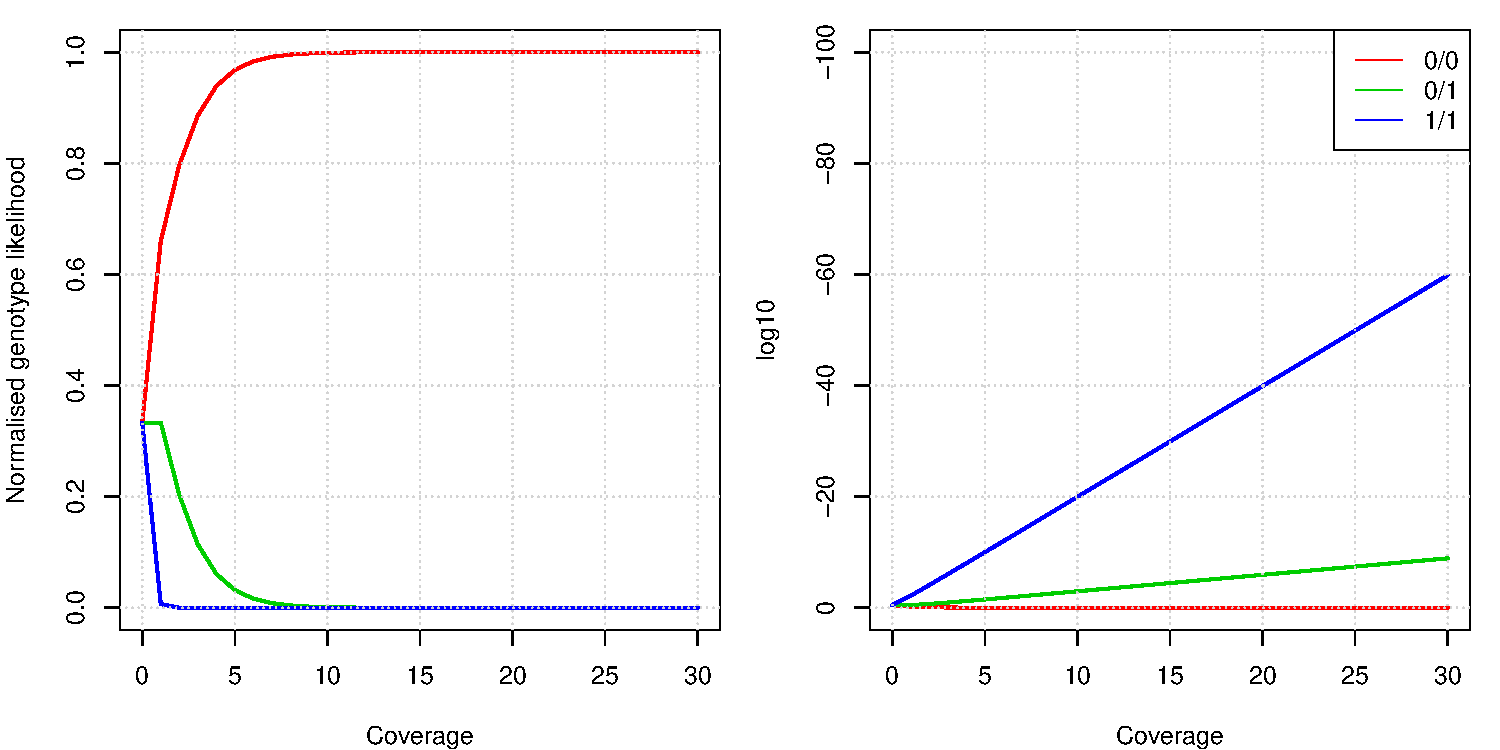
\includegraphics[width=\textwidth]{figure1}
    \caption{Example of how the GLs behave as a function of depth when $\epsilon=0.01$}
  \end{center}
\end{figure}

\end{document}
